\chapter{Architecture}

\section{System Overview}
Basically, the architecture consists of two main components namely the broker and
the client, whereas the client can act as producer, consumer or both. The broker
is a server which only reacts to requests that are sent from clients. Every
request contains an API key which the broker uses to determine which action it
has to do (e.g. persist produced message or consume message). For each valid
request the broker sends back a corresponding response to the client which
either includes the fetched data or an error code. The broker never communicates
with a client without a request.

\begin{figure}[H]
    \centering
     \begin{sequencediagram}
        %\newthread{broker}{Broker}
         \newinst[3]{client}{Client}
         \newinst[3]{broker}{Broker}
        \begin{messcall}
            {client}{(1) Send Request}{broker}{}
        \end{messcall}
        \begin{messcall}
            {broker}{(2) Do Action}{broker}{}
        \end{messcall}
        \begin{messcall}
            {broker}{(3) Send Response}{client}{} 
        \end{messcall}
     \end{sequencediagram}
     \caption{Basic communication between client (producer or consumer) and
     broker}
\end{figure}

\subsection{Producer Client}
Depending on which API key a request contains, a client can act either as
producer or consumer. In the case of a producer client, the following main steps
are made.
%For demonstrating the architecture of this project we implement an architecture
%prototype which shows basic functionality of producing a message from a client A
%omplete) a  topic specific log at the broker and in turn consuming it from another
%client B. It fully implements the produce and fetch request with their
%appropriate responses of the Kafka protocol for communication over network.
%Therefore the producer and consumer clients are compatible with original Apache
%Kafka broker.

%The functionality of the architecture prototype can be split in two cases.
%Case one covers producing a message and persisting in the brokers log:
\begin{figure}[H]
    \centering
    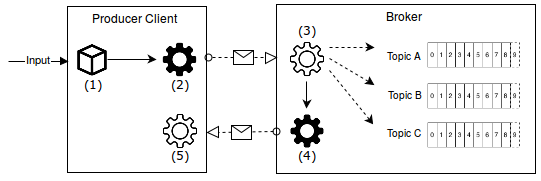
\includegraphics[width=0.8\textwidth]{images/concept_producer.png}
    \caption{Concept of Architecture Prototype Part I}
    \label{fig:conept-producer}
\end{figure}

\begin{description}
    \item [(1)] 
        {Packing Produce Request: Getting input data to protocol conform data structure.}
    \item [(2)] 
        {Serializing and send Produdce Request: Encoding data structure to an
            binary  string and transmit over a tcp socket to the broker.}
    \item [(3)] 
        {Parsing and Handling Produce Request: Broker receives the binary string
            and parse it back to the appropriate data structure. The request
            handler of the  broker checks the API Key of the request. If it is a
            produce request, the containg message will be written to the
            appropriate topic log.}
    \item [(4)] 
        {Send Produce Response: A response is packed, serialized and transmitted
            back to the client. The response contains an error code which has
            the value 0 if everything worked well otherwise another value for a
            specific problem. }
    \item [(5)] 
        {Parse Produce Response: Producer client receives a binary string and
            parses it to valid response data structure }
\end{description}

\subsection{Consumer Client}
Like Apache Kafka, our architecutre is based on pull-based consumption. The consumer
fetchs it desired messages through requesting it at any time. 

\begin{figure}[H]
    \centering
   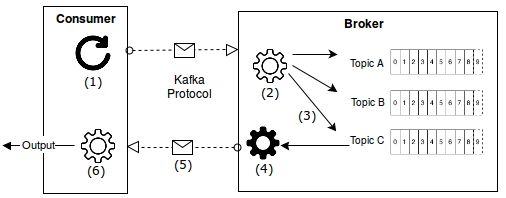
\includegraphics[width=0.7\textwidth]{images/concept_consumer.png}
    \caption{Concept of Architecture Prototype Part II}
    \label{fig:concept-consumer}
\end{figure}

\begin{description}
    \item [(1)] 
        {Continously send fetch request: Consumer client sends fetch
        requests in configurable intervall as binary string to the broker. } 
    \item [(2)] 
        {Parsing and handling fetch request: Broker receives the binary string
            and parse it back to the appropriate data structure. The request
            handler of the broker checks the API Key of the request. If it is a
            fetch request, the broker reads messages of the requested topic and
            packs it to a fetch response. message will be written to the
            appropriate topic log.}
    \item [(3)] 
        {Send fetch response: The fetch request which contains the requested
        messages is send back to the consumer client.}
    \item [(4)] 
        {Parse Response:Consumer client receives a binary string and parses it
        to valid response data structure }
\end{description}

\section{Design decisions}
\subsection{Protocol}
For communicating over network we implement a binary protocol based on tcp.
Because we use Apache Kafka as benchmark for this project and we want to provide
compatibility to existing Kafka clients, we decided to fully implement the Kafka
Protocol version 0.8.x \todo{ref}. It differ in six APIs which each of it is
defined with a request-response message pair. The client initiates a socket connection and then
writes a sequence of request messages and reads back the corresponding response
message. 

TODO: What design desicions we made regarding the protocol? (Types, Serializer,
Parser). 

\subsection{Separation} 
\label{sec:separation}
Both, the client and broker component need to use the same underlying protocol for
communication. Therefore we provide a third component which fully implements the Apache Kafka
protocol \todo{ref} and provides the appropriate functions and types as library.
This component fully separates the clients from the broker. It also allows to
use the clients with other Kafka based broker implementations, especially Apache
Kafka itself. 

To support interoperability we want to simplify the implementation of a broker
client. Therefore we provide a client library which provides functionalities to
easily implement a Haskell client. The goal of this, is to be able to
setup a client without knowing too much details about the Apache Kafka protocol
itself. We therefore provide separate types to construct a message very easily.
In the background we then pack the input to the appropriate Request/Response
Message. 

\begin{figure}[H]
    \centering
    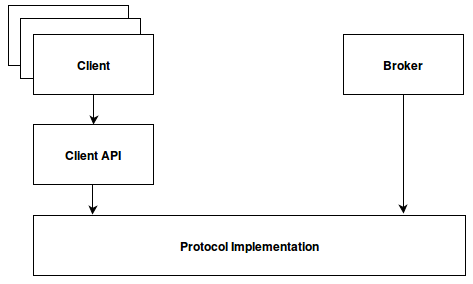
\includegraphics[width=0.55\textwidth]{images/architecture-components.png}
    \caption{Separation of code}
    \label{fig:architecture-components.png}
\end{figure}

\subsection{Consumption Model}
TODO: All requests are initiated by the client, and result in a corresponding
response message from the server

\subsection{Broker Layering}
We decided to divide the broker server application into three subsystems to
clarify the program flow from receiving data from network to handling the
requests and accessing the message log. 
\subsubsection{Network Layer}

TODO: introduction to tasks of networking layer, then ref to socket server implementation

\begin{figure}[H]
    \centering
    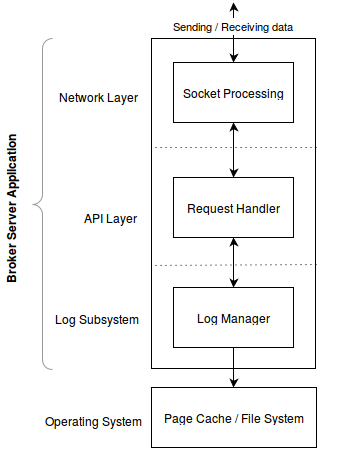
\includegraphics[width=0.3\textwidth]{images/design-subsystems.png}
    \caption{Three subsystems of broker server application}
    \label{fig:architecture-subsystems.png}
\end{figure}

\subsubsection{API Layer}

TODO: introduction to tasks of api layer, then ref to request and error handling

\subsubsection{Log}

TODO: introduction to tasks of log subsystem, then ref to persistance section



